\documentclass{article}
\usepackage{amsmath, amsthm, amsfonts, geometry, graphicx, blindtext}
\usepackage{natbib}
\usepackage{hyperref}
\usepackage{setspace}
\usepackage{indentfirst}
\usepackage{tabularx, booktabs, caption, float}
\usepackage{tikz, pgfplots}
\usepackage{multicol}
\usepackage{titlesec}
\usepackage{xcolor}
\pgfplotsset{compat=1.18, width=0.9\linewidth}

\captionsetup[table]{singlelinecheck=false, justification=raggedright, format=plain}

\setlength{\parindent}{1cm}
% \fontsize{8pt}{10pt}\selectfont
% \spacing{1.5}

\newgeometry{
    top = 0.75in,
    inner = 0.75in,
    outer = 0.75in,
    bottom = 0.75in
}

\renewcommand{\thesection}{\Roman{section}}
\titleformat{\section}
    {\fontsize{1em}{1.2em}\bfseries\centering\uppercase}{\thesection}{1em}{}

\renewcommand{\thesubsection}{\arabic{section}.\arabic{subsection}}
\titleformat{\subsection}
    {\fontsize{1em}{1.2em}\bfseries}{\thesubsection}{1em}{}

% \renewcommand{\thechapter}{\Roman{chapter}}

% For the chapter heading that has the title name after the line of the chapter number
% \titleformat{\chapter}[display]
    % {\fontsize{2em}{2.2em}\bfseries\centering}{\chaptertitlename\ \thechapter}{1em}{}
    % {\fontsize{2em}{2.2em}\bfseries\centering}{\thechapter}{0.25em}{}

% For the chapter heading that have the title name and chapter number in the same line
% \titleformat{\chapter}[hang]
%   {\fontsize{2em}{2.2em}\bfseries\centering\uppercase}
%   {\chaptertitlename\ \thechapter}{1em}{}


\title{{\Huge Lab Exercise 2}\\{\small CS ELEC 2C}}
\author{Alessandro Andrei Araza \and Joshua Kyle Entrata}
\date{\today}

\begin{document}

    \maketitle

    \begin{abstract}
        % TODO: Abstract here
        ABC Supermarkets needs to do an analysis of whether or not their previous customers will accept their year-end sale of offering a gold membership for a cheaper price of \$499 compared to \$999 on the usual days. They wanted to know if their phone call campaigns would accepted by making a predictive model to classify which customers would purchase the offer. For implementation, logistic regression, support vector machines, naive bayes, decision trees, and k-nearest neighbors models were used to evaluate the dataset. Models had undergone cross-validation to ensure the consistency of reuslts. It was found throughout all of the models that someone's year of birth, their purchases (regardless of at the store, online, or what did they buy), and their marital status had a play at determining if they would accept the offer. 

        \vspace{0.5\baselineskip}
        \noindent
        % \textbf{Keywords:} TODO: keywords
    \end{abstract}

    \begin{multicols}{2}
        \section{Introduction}

% TODO: intro

Supermarkets, like any other business, needs to meticulously and careful plan out their business decisions because one wrong move could result in millions of losses in revenue. However, risky business decisions are what create the most capital, popularity, and overall growth of the company as these decisions create new avenues by attracting more customers or strengthen old ones. Risky business decisions does not always need to be a gamble, there are a lot of ways to turn it into a calculated risk; this would in turn allow a company to somewhat have an idea of their possible gains, loss, and approach to the risks. The most traditional method for calculating risks is from listening to the veterans of the business. However, there are now more effective ways to help business decisions with one leveraging data. Data and machine learning can help by providing models that predict the outcomes to an accurate level that would help in the approach of risky business decisions. 

\subsection{Problem and Dataset}

The lab exercise is provided a dataset that contains various personal information a customer. To be more specific the dataset contains the columns as shown in table \ref{tab:columns}.

The Response column will be the target of the machine learning models. To interpret, the goal of the machine learning models was to predict which customers accepted the offer in the last campaign. Doing so would give ABC Supermarkets an idea who might be willing to accept the offer of their year-end sale campaign for existing customers. 

\begin{table}[H]
    \caption{Table of the dataset attributes and their data type}
    \label{tab:columns}
    \begin{tabularx}{\linewidth}{l>{\centering\arraybackslash}X}
        \toprule
        Column & Data type \\
        \midrule
        ID & int64\\
        Year\_Birth & int64\\
        Education & object\\
        Marital\_Status & object\\
        Kidhome & int64\\
        Teenhome & int64\\
        Dt\_Customer & object\\
        Recency & int64\\
        MntWines & int64\\
        MntFruits & int64\\
        MntMeatProducts & int64\\
        MntFishProducts & int64\\
        MntSweetProducts & int64\\
        MntGoldProds & int64\\
        NumDealsPurchases & int64\\
        NumWebPurchases & int64\\
        NumCatalogPurchases & int64\\
        NumStorePurchases & int64\\
        NumWebVisitsMonth & int64\\
        Response & int64\\
        Complain & int64\\
        \bottomrule
    \end{tabularx}
\end{table}


        \section{Methodology}

% TODO: method

        \section{Experiments}

% TODO: experiments

\subsection{EDA}

EDA provides an overview of what could be done to the data to improve the models' performance. 

\subsubsection{Data Profiling and Malformed Entries}

All of the columns and their data types can be seen at table \ref{tab:columns}. When checking for null values, all other columns are free from it other than \texttt{Income}. Upon inspection, there seems to be no connection with all the other attributes of the entries with null valued `Income`. As far as inspection and analysis goes, they seem to just be malformed entries. 

\texttt{Marital\_Status} also has multiple entries that could be thought of as different, similar, or sometimes even a malformed entry. In the list of unique values for the column, the values are \texttt{Divorced, Single, Married, Together, Widow, YOLO, Alone, Absurd}. Upon listing the value counts, \texttt{Alone, YOLO, Absurd} have very few entries which could be considered as outliers. There are been thoughts of merging some of these entries to the other entries with bigger value counts; e.g. \texttt{Single} would adopt the records with \texttt{Alone}, etc. However the problem lies wherein there is no way to deduce their backgrounds and whether or not the adopting categories should take in the outliers. To further explain, there is no way to tell if a record that is \texttt{Alone} might have came from a divorced background or if they simply are single. However further explanation of the choice between data integrity and model performance would come in later in experimentations

\subsubsection{Univariate Analysis}

The skew and imbalance of data attributes can be seen upon further isolated inspection. Firstly, \texttt{Income}'s central tendencies at table \ref{tab:income desc}

To put into perspective figure \ref{fig:income hist} shows the distance of the max value from the mean of the distribution with a skewness of 6.763487372811116

Depending if the models are robust to outliers, they will be removed, experimentations will further explain these phenomena

\begin{table}[H]
    \caption{Income column's descriptive statistics}
    \label{tab:income desc}
    \centering
    \begin{tabularx}{0.7\linewidth}{l>{\raggedleft\arraybackslash}X}
        \toprule
        Statistic & Value\\
        \midrule
        count & 2216 \\
        mean & 52247.251354\\
        std & 25173.076661\\
        min & 1730\\
        25\% & 35303\\
        50\% & 51381.5\\
        75\% & 68522\\
        max & 666666\\
        \bottomrule
    \end{tabularx}
\end{table}

\begin{figure}[H]
    \centering
    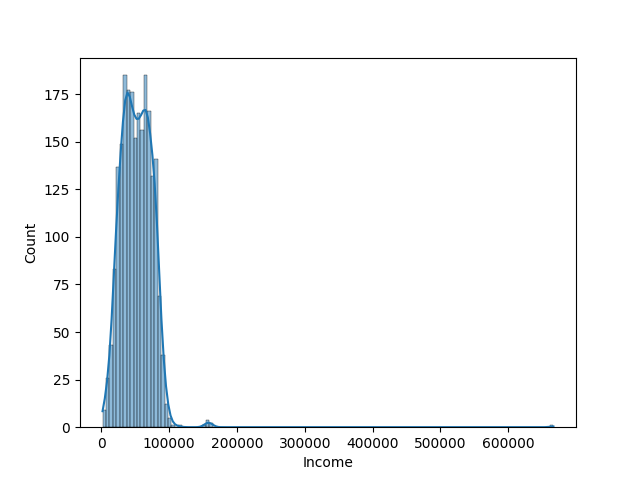
\includegraphics[width=\linewidth]{figures/income_histplot.png}
    \caption{histogram of Income values}
    \label{fig:income hist}
\end{figure}

On the other hand for \texttt{Education} While it could be considered that the \texttt{Basic} records are outliers, removing them may misrepresent the dataset.

% \begin{figure}[H]
%     \centering
%     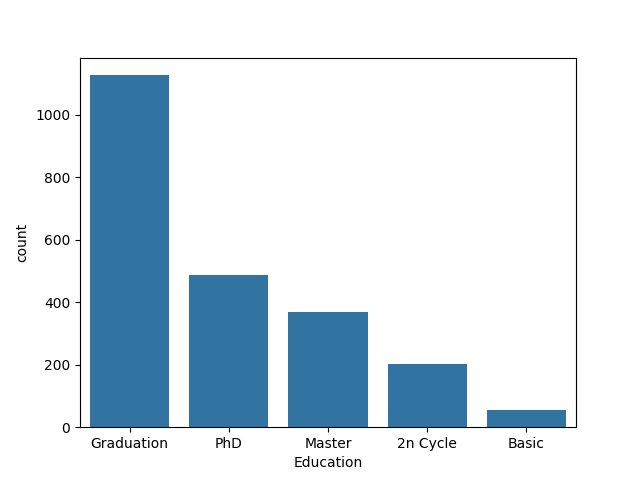
\includegraphics[width=\linewidth]{figures/education_barplot.png}
%     \caption{Bar plot of value counts of the Education column}
%     \label{fig:educ bar}
% \end{figure}

\subsubsection{Bivariate Analysis}

The relationships of attributes to each other are also worth considering to look at. Given that a lot of the analysis of these attributes would later be interpreted by the models which will be seen at the discussion.

Looking at the scatterplot for the income per year of birth, ignoring the outliers, it seems that there seems to be an equal distribution for each year. Looking around the years 1970 to 1980, there seems to be a few entries where the recorded income is higher than the usual. 

\begin{figure}[H]
    \centering
    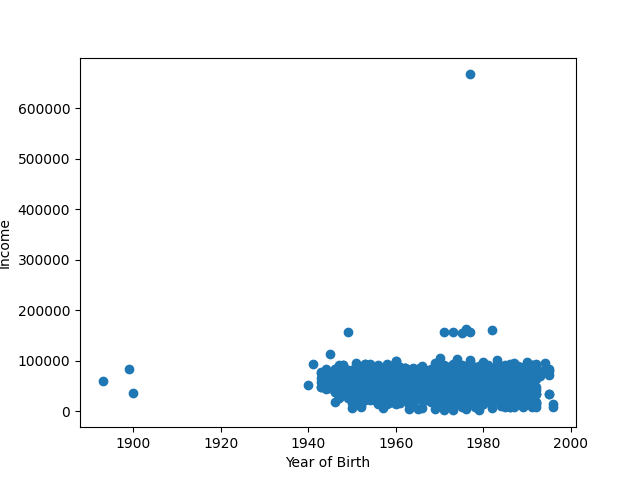
\includegraphics[width=\linewidth]{figures/income_per_yob.png}
    \caption{Scatterplot of income per year of birth}
\end{figure}

Regarding education, when categorized and calculated for central tendencies, \texttt{Basic} provides the lowest average income, while a \texttt{PhD} provides the highest average. However, according to table \ref{tab:educ mean std}, Basic education seems to be the most stable when it comes to delivering a salary based on the standard deviation. PhD education, although high in the average salary, is also very high in standard deviation. This could be seen at the $min$ and $max$ of each category where the minimum income of someone with PhD degree can be as low as 4023 while someone with basic education can be sure to have a salary that is atleast 7500.

\begin{table}[H]
    \caption{Descriptive statistics for each unique value in the Education column}
    \label{tab:educ mean std}
    \begin{tabularx}{\linewidth}{l|>{\centering}X>{\centering}X>{\centering}X>{\centering\arraybackslash}X}
        \toprule
        Education & $\bar x$ & $\sigma$ & min & max \\
        \midrule
        2n Cycle & 47633.19 & 22119.08 & 7500 & 96547\\
        Basic & 20306.26 & 6235.07 & 7500 & 34445\\
        Graduation & 52720.37 & 28177.19 & 1730 & 666666\\
        Master & 52917.53 & 20157.79 & 6560 & 157733\\
        PhD & 56145.31 & 20612.98 & 4023 & 162397\\
        \bottomrule
    \end{tabularx}
\end{table}


\subsection{Preprocessing}

\subsubsection{Data Cleaning} 

    2.2.1.1 Handling null values. During the preprocessing phase, one of the important steps to was to address the null values, particularly within the \texttt{Income} column. Several solutions were considered for dealing with the null values in this column. 

    First, it was proposed to fill null values with the median of their respective groups. This method imputes missing values with the meadian income of similar groups based on other features, such as \texttt{Education} or \texttt{Marital\_Status}. But after examining the relationship between \texttt{Income} and these categorical variables, we observed weak correlations:
        - For \texttt{Education} levels, the correlation coefficients ranged from -0.200576 to 0.081552 which indicate a weak relationship between these features.
        - Similarly, for \texttt{Marital\_Status}, the correlation coefficients ranged from -0.025843 to 0.0031706, also suggesting a weak relationship between these features.

    Given these weak correlations, imputing null values based on the meadian of their respective groups might not provide a meaninful impact on the models. It may also introduce inaccuracies into the dataset because neither \texttt{Education} nor \texttt{Marital Status} strongly predict \texttt{Income}.

    Second, another approach for these missing \texttt{Income} values was to fill it with 0. This method can be justified if a null value represents customers; lack of income. However, this assumption is generally not accurate for most of the datasets. It could significantly skew the data distribution and inflate the count of customers' with zero income. Therefore, filling null values with zero was viewed as not optimal due to its potential to misrepresent the information of the customers in the dataset.

    Lastly, given the drawbacks of the first two approaches, it was decided to remove rows with null values. This decision was made by considering the analysis done in the features and preserving the integrity of the data. Although this approach may result in a smaller dataset, it ensures that reliability and complete information, which reduces the potential for skewed results and maintain data quality.

    2.2.1.2 Handling Outliers. Outliers were observed within the \texttt{Income}, \texttt{Mnt.*}, and \texttt{Num.*} columns during the exploratory data analysis phase. Visualization tools, such as kernal density estimate and scatter plots, indicated the presence of extreme values that could potentially affect the modelling. The following algorithm for removing outliers on continuous variables was implemented:

    % TODO: apply the picture of the remove_outliers function

    By applying this algorithm, it ensures that the analysis is not skewed by extreme values, leading to more accurate results and improves the quality of the models.

\subsubsection{Feature Engineering}

    2.2.2.1 Creating Total Children Feature. A new column called \texttt{Total\_Children} was created by summing up the \texttt{Kidhome} and \texttt{Teenhome} columns. This new feature provides anothger information for the total number of children in each customer's household, which could help in understanding the purchasing behavior or creating new marketing strategies based on this new feature.

    2.2.2.2 Removing Unrealistic Customers based on Year of Birth. During the exploratory data analysis phase, a number of outliers in the \texttt{Year\_Birth} column was recognized, that is why the dataset was filtered to only include records where the column value is 1940 or later. This ensures a realistic age range for customers.

    2.2.2.3 Converting dates to Datetime and validation. The values in the \texttt{Dt\_Customer} column was converted to a datetime type. To ensure the dataset contains valid dates, checks were implemented to verify that there are no future dates and that the year of birth is not later than the year of becoming a customer.

    2.2.2.4 Calculating Days Since Becoming a Customer. The number of days since the date of becoming a customer up to the current date was calculated. This new feature, \texttt{Days\_Since\_Customer}, was created to help in understanding the customer tenure, which can be important in models to predict customer loyalty.

    2.2.2.5 Cleaning Marital Status Values. There are two approaches proposed in cleaning these values. At first, dropping the rows with \texttt{Marital\_Status} values of \texttt{YOLO}, \texttt{Absurd}, and \texttt{Alone} was considered. But this approach may possibly negatively affect the integrity of the data. That is why replacing this status labels with \texttt{Single} was done to maintain data size and integrity. This homogenization helps in reducing the variability within the data. This helps in decreasing the number of different values which can help in making the analysis more straightforward.

\subsubsection{One-Hot Encoding}

Columns \texttt{Education} and \texttt{Marital\_Status} are categorical values. While there is an option to use factorization for these data, there is a risk of misinterpretation since the factorized values could imply that one number has a greater value than the other, which could lead to misinterpreation during the modelling process. 

\subsubsection{Interaction Features}

Given the statistical evidence from the ANOVA test - F = 2.815 for \texttt{Kidhome} and F = 4.461 for \texttt{Teenhome}, with p-values well below the 0.05 significance level - during the explroatory data analysis phase, the results shows strong evidence that \texttt{Marital\_Status} significantly impacts the number of children and teenagers in a household. This suggests that marital status may interact with household composition that may provide a meaningful impact on the model. To quanitify these relationship, interaction features were created by multiplying each one-hot encoded marital status column by \texttt{Kidhome} and \texttt{Teenhome} to create new interaction columns. These interaction features can potentially imrpove the performance of the models. They allow models to provide deeper insights on how households interact with the customers' marital status.

\subsubsection{Feature Selection}

The objective was to construct a predictive model to classify customers who might purchase the new year-end sale offer based on variables that may have a direct or indirect impact. Through careful analysis, there are columns that were dropped, such as \texttt{ID}, \texttt{Dt\_Customer}, \texttt{Kidhome}, and \texttt{Teenhome}. 

The \texttt{ID} contains unique identifiers for each record which are typically irrelevant to the outcome of predictive models. The date when the customer joined have been used to derive new feature, \texttt{Days\_Since\_Customer}, therefore the original date is no longer necessary for the modelling. The columns \texttt{Kidhome} and \texttt{Teenhome} were used to create interaction features and new feature, \texttt{Total\_Children}. Retaining these original columns might be redundant and could even introduce noise.

Additionally, interaction features were introduced by  using one-hot encoded marital status and variables like \texttt{Kidhome} and \texttt{Teenhome}. Removing the original one-hot encoded columns can help in avoiding multicollinearity and potentially improve the performance of the models due to reduced dimensionality and complexity.

\subsubsection{Scaling}

Large distance between features can negatively affect the model's performance. For example, the \texttt{Income} value are in thousands, while the other variab;es, especially those that have underfone one hot encoding only range in single digits. With the use of feature scaling, this would help the models in dealing with values that are too distant in range.

The use of \texttt{StandardScaler} helps prepare the dataset for many machine learning algorithms, particularly those sensistive to the scale of features, such as Support Vector Machines (SVM), and K-Nearest Neighbors (KNN). 

\subsubsection{Polynomial Feaures}

While adding more features to a model doesn't equate to better performance, there is still a significant effect to a machine learning model when utilized correctly. The introduction of polynomial features would create a polynomial based on a single feature where each monomial would become an input in the model. The use of \texttt{interaction\_only=True} extends the datset with features that represent the products of pairs of original features. This is based on assumption that the relationship between some variables could exhibit boosting when combined. By integrating polynomial feature, it can help the models with a comprehensive framework capture more complex relationships within the data.



        \section{Results and Discussion}

% TODO: RnD
Due to the nature of the experimentation, there are five versions each implemented machine learning model, each with different hyperparameters. However, for the interpretation and discussion of results, only the best performing model are taken into consideration. 

\subsection{Logistic Regression results}

Due to the polynomial features, there were 465 columns fed into the models, because of this, it's best to instead take note of the most significant coefficients from the model. Looking at table \ref{tab:lr top5 coef}, it can be observed that the most significant features are all interaction features.

\begin{table}[H]
    \caption{Top 5 Features in the logistic regression model}
    \label{tab:lr top5 coef}
    \begin{tabularx}{\linewidth}{l>{\centering\arraybackslash}X}
        \toprule
        Feature & Value \\
        \midrule
        MntFruits \\ A\_Marital\_Status\_Single\_Kidhome & 0.979750 \\
        \midrule
        MntMeatProducts \\ A\_Marital\_Status\_Married\_Teenhome & 0.952025 \\
        \midrule
        MntWines \\ A\_Marital\_Status\_Together\_Teenhome & 0.844306 \\
        \midrule
        Education\_Master \\ A\_Marital\_Status\_Single\_Kidhome & 0.814164 \\
        \midrule
        MntWines \\ NumWebPurchases & 0.763514 \\
        \bottomrule
    \end{tabularx}
\end{table}

It is observed that people who bought fruits and are married with a kid at home are very likely to respond and accept the offer. The likeliness to accept the offer can also be seen with married people with a teen at home who also bought meat products in the last two years, people that live with someone (\texttt{Together} marital status value) that buys wines with a teen at home, single people who achieved masters education with a kid at home, as well as people who bought wines in the last two years that also bought products at the company's website.

\subsection{SVM}

Since the best model tested in the SVC models is a linear model, it can be interpreted that the coefficients to understand how the model has learned. Table \ref{tab:svm top5 coef} shows a lot of similarity with the top five coefficients of the linear regression model. 

\begin{table}[H]
    \caption{Top 5 features in the SVM model}
    \label{tab:svm top5 coef}
    \begin{tabularx}{\linewidth}{l>{\centering\arraybackslash}X}
        \toprule
        Feature & Value \\
        \midrule
        MntWines NumWebPurchases & 0.904773 \\
        A\_Marital\_Status\_Married\_Kidhome \\ A\_Marital\_Status\_Married\_Teenhome & 0.804857 \\
        MntFruits \\ A\_Marital\_Status\_Single\_Kidhome & 0.803837 \\
        NumWebVisitsMonth \\ A\_Marital\_Status\_Single\_Kidhome & 0.769760 \\
        Recency \\ Days\_Since\_Customer & 0.733147 \\
        \bottomrule
    \end{tabularx}
\end{table}

As it turns out, the support vector machine model's top five coefficients has two features similar to the top five of the linear regression model. This would make sense because although they are different machine learning models, grid search algorithm has decided that the best hyperparameters for the SVM included that the svm should use a linear kernel. This would imply that the data is much akin to being linearly separable. Table \ref{tab:svm top5 coef} implies the same ideas as it did for the features that were also in table \ref{tab:lr top5 coef}. For the features unique to table \ref{tab:svm top5 coef}, they simply imply that people who are married with children and teenagers at home, single with a kid at home that visits the company's website in the past month, and people who haven't bought in a while (high \texttt{Recency} value) that are also long standing customers (high \texttt{Days\_Since\_Customer} value) are more willing to respond and accept the offer.

It is a bit difficult to interpret the support vectors found by the SVM. Mainly because any aggregation to these found support vectors are only slightly different to the aggregations found in the original dataset. For example, the average \texttt{Year\_Birth} for the dataset is 1970.325371 while the average for the support vectors is 1970.030303; this is reflected to the other attributes even with different aggregation methods, whether it is the average, standard deviation, etc. the results only vary by a few units. This could be explained by the idea that maybe much of the data points are closer to decision boundary than expected. According to the model there are a total of 198 support vectors found in the dataset; 131 for no responses, and 67 for the responses. To put into perspective, out of the total 971 entries in the training set, 131 are support vectors, that is about 20.3\% of the training set. 

\subsection{Naive Bayes}

According to the implemented Bernoulli Naive Bayes, the log probability of a 0 response (not accepted) is -0.09726884, while a 1 response (accepted the offer) is -2.3785168. This means that the chance of accepting the offer is much lower in probability compared to rejecting it which would make sense given there is a heavy imbalance in the dataset where 1101 responses are 0 while only 113 entries have a response of 1.

When analyzing the log probability of a feature, the values imply the probability of a feature for a given class, i.e. $P(x_i \mid y)$. Just like the analysis of coefficients at the logistic regression and SVM models, there is too much features to be able to show them all. So, just as before, it is best to just look at the highest scoring (or alternatively, the lowest scoring) of the feature log probabilities.

\begin{table}[H]
    \begin{tabularx}{\linewidth}{l>{\centering\arraybackslash}X}
        \toprule
        Feature & $Log P(x_i \mid y)$ \\
        \midrule
        Year\_Birth & -0.624380 \\
        \midrule
        Year\_Birth Recency & -0.641402 \\
        \midrule
        NumCatalogPurchases \\ Days\_Since\_Customer & -0.650023 \\
        \midrule
        NumCatalogPurchases & -0.650023 \\
        \midrule
        Recency & -0.650023 \\
        \bottomrule
    \end{tabularx}
\end{table}

\subsection{Decision Trees}

\subsection{K-Nearest Neighbor}

        \section{Conclusion}

% TODO: conc

    \end{multicols}

    % Include in the bibliography all that was uncited
    % \cite{mitlohner_characteristics_2016}
    %
    % this is a reference \citep{gaines_emotional_1983} vs the regular reference \cite{gaines_emotional_1983}.
    % \nocite{*}

    % \newpage
    % \bibliographystyle{apalike2}
    % \bibliography{citations} % Put the file name only of the .bib files
    % https://zbib.org/59898e1965a74f2f9d57017519db0564

\end{document}
